\documentclass{article}
\usepackage[utf8]{inputenc}
\usepackage{geometry}
\geometry{a4paper, margin=1in}
\usepackage{graphicx}
\usepackage{hyperref}
\usepackage{float}
\usepackage{datetime}

\hypersetup{
	colorlinks=true, 
	linkcolor=blue, 
	urlcolor=blue, 
	citecolor=blue
}

\setlength{\parindent}{0pt} % Disable indentation for new paragraphs

\title{Data Wrangling \& Visualization: First Checkpoint \\
 \textbf{Interactive Visualization of \texttt{UMAP} Algorithm on User Data}}
\author{Nikita Zagainov, Dmitry Tetkin, Nikita Tsukanov}
\date{\monthname[\the\month] \the\year}

\begin{document}

\maketitle

\section{Results Of Data Collection \& Preprocessing}

As it was stated in project proposal, our project 
has little data processing, this is why our main focus
during this checkpoint was on algorithm implementation.

\section{Our Work So Far}

During the first spring, our team adapted the original 
\href{https://arxiv.org/abs/1802.03426}{UMAP} implementation
to be able to stream intermediate results of the descent.
Our contribution can be found in  
\href{https://github.com/V1adych/umap}{this repository}.

\section{Demo}

\begin{figure}[ht]
	\centering
	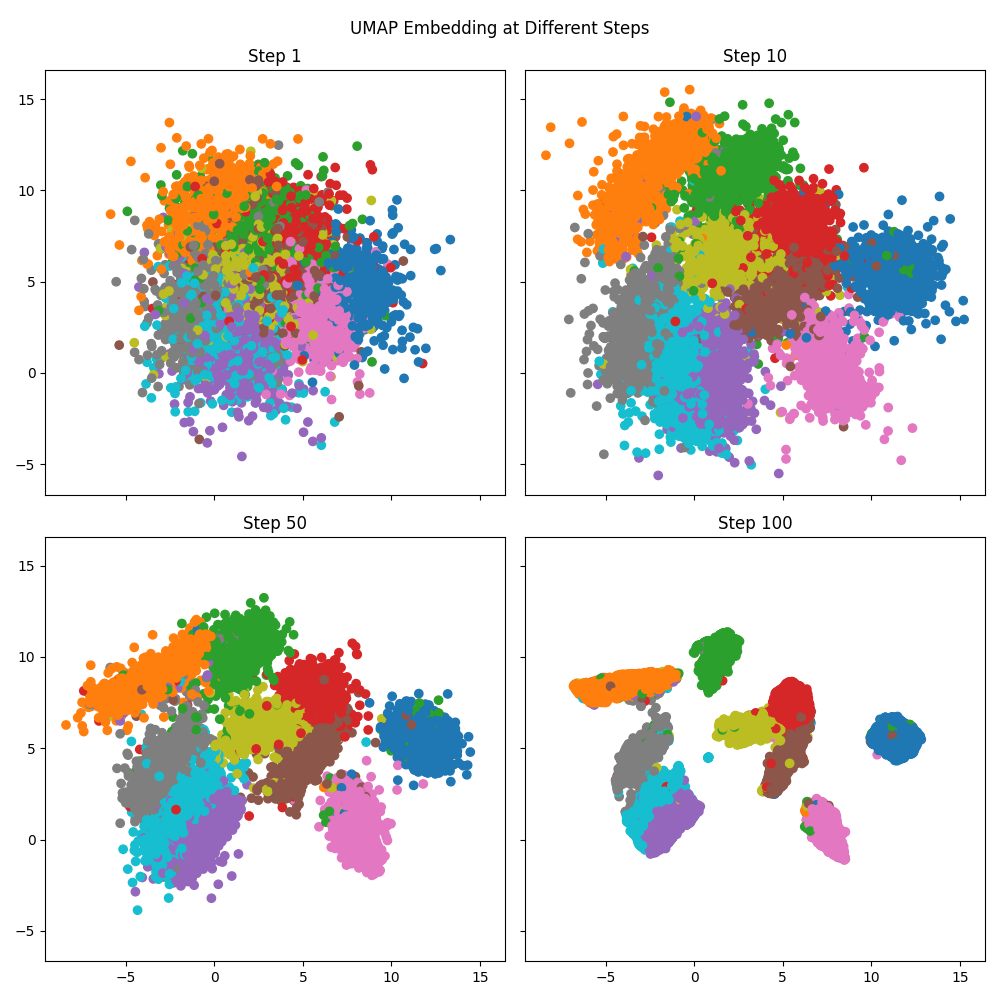
\includegraphics[width=0.8\linewidth]{assets/umap_steps.png}
	\caption{UMAP Steps Visualization on MNIST dataset. 
	Different colors correspond 
	to different labels (digits), algorithm had no access to true 
	labels during learning embedding}
	\label{umap_steps}
\end{figure}

Figure \ref{umap_steps} shows the visualization of the 
UMAP algorithm applied to 
\href{https://yann.lecun.com/exdb/mnist/}{MNIST} dataset.
The code to reproduce this visualization can be found in
our repository, in the \verb|notebooks/visualization_example.ipynb| 
notebook.


\end{document}